\section{Data Exploration}\label{sec:data-exploration}

\subsection{Scope and distributions}

The supplied dataset contains 870 responses from 290 respondents, each answering for Baseball, Basketball and Soccer. All new descriptive results below use only the recorded exploration training subset: 232 respondents and 696 responses, with 232 responses per class. The remaining 58 respondents are excluded from this new exploration. These are development partitions, subject to the historical exposure limitation described below.

The inputs comprise one bounded numeric ease score, three ordinal Likert items (strategy, injury and individual brilliance), three multi-select questions (venue, season and music), four free-text questions (food, colour, song and feelings), and a free-text payment amount. The transformation yields 73 predictors: five numeric or ordinal values and 68 binary flags. Respondent ID and the target label are excluded.

Ease spans 0-10 (mean 5.40, sample SD 2.32). The mean Likert scores are 3.78, 3.50 and 3.41, respectively; agreement is the modal response for all three. Multi-select indicators can co-occur; summer is the most frequently selected season. Median answer lengths for food, colour, song and feelings are 16, 5, 17 and 9 characters, with long right tails. Fixed keyword flags match 95.5\% of food, 96.0\% of colour and 89.8\% of feelings rows; song-category flags match only 35.6\%. Unmatched language remains a limitation.

Baseball has a lower mean ease score (4.06) than Basketball (6.01) or Soccer (6.14). Indoor venues occur in 96.1\% of Basketball answers, versus 24.6\% of Baseball and 61.2\% of Soccer answers. The Waka song flag occurs in 57.8\% of Soccer answers and none of the other two classes. These patterns support a linear softmax baseline and trees that capture thresholds and interactions; a random forest can reduce the variance of an individual tree. They do not establish predictive accuracy.

\subsection{Missing values and unusual amounts}

There are 15 blank song answers (2.2\%), nine blank food answers (1.3\%), and seven or eight blanks (1.0-1.1\%) for every other question. Literal N/A and none answers are preserved as content; this differs from automatic CSV missing-value detection in the proposal. No observed ease score is outside 0-10, and no nonblank Likert or multi-select response is unrecognized.

\begin{figure}[ht]
\centering
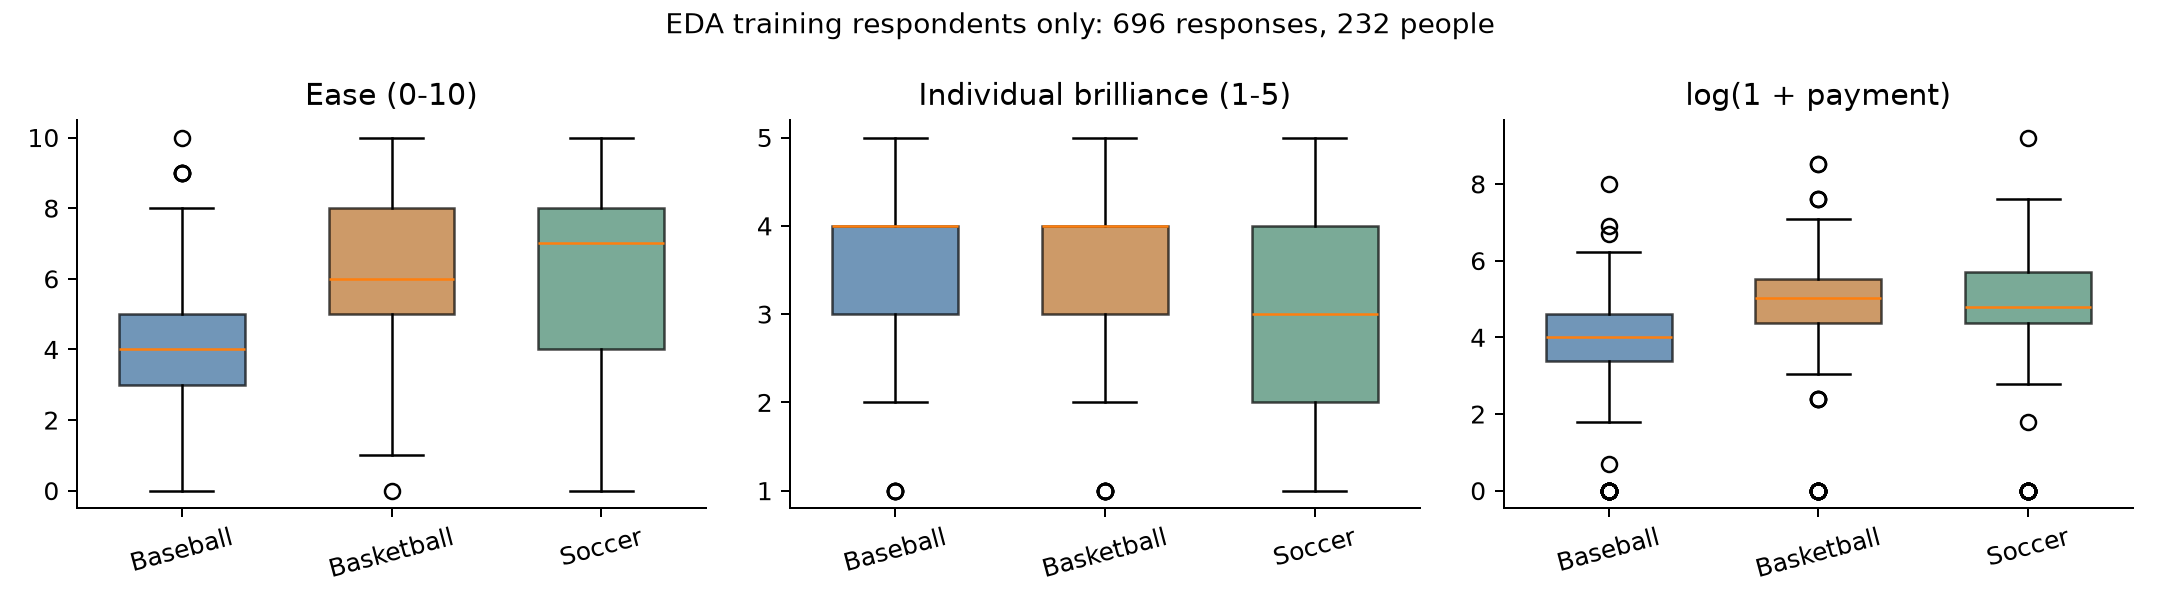
\includegraphics[width=\linewidth]{development/eda/figures/numeric_by_class.png}
\caption{Class-conditioned distributions in the 696-row exploration training subset. Ease and payment differ by class, but distributions overlap.}
\label{fig:training-distributions}
\end{figure}

\subsection{Preprocessing shared by the actual candidates}

The fixed definitions apply to softmax regression, decision tree and random forest. Text is normalized for Unicode, whitespace and case. Likert responses map to integers 1-5, with missing or unrecognized entries set to neutral (3). Venue, season and music use 7, 4 and 10 multi-hot columns; unknown options activate no known option. Food, colour and feelings use 24, 10 and nine fixed regex indicators. Songs use three category flags and a separate named-song flag. Blank or unmatched text produces zero keyword flags. Historical keyword definitions are preserved rather than expanding them after inspecting new validation responses.

Ease is clipped to 0-10 and missing values use the training median (5 in this exploration). The payment parser accepts a nonnegative amount, k suffix, explicit refusal (0), simple written number or unambiguous ascending range (midpoint). It does not average unrelated amounts. Here it accepts 597 numeric answers, 30 ranges, 27 refusals and three written numbers. The remaining 39 answers (5.6\%) are blank, ambiguous, foreign-currency or unparsed text and use the training median (100). Parsed amounts reach 10,000; 81 exceed the usual 1.5-IQR fences. Valid amounts are retained and transformed with log(1 + amount), reducing skew without deleting respondents (transformed mean 4.29, SD 1.88, with a spike at zero).

For softmax regression, ease, the three Likert values and log-payment are standardized using training means and population standard deviations; binary flags remain 0/1. A constant column uses scale 1. Trees use the unscaled values. Every inner or outer training partition must fit its own medians and scaling state, then apply that saved state unchanged to validation rows. The exploration state is not a cross-validation or final deployment state.

\subsection{Respondent separation and historical exposure}

Preliminary exploration informed the fixed keyword definitions before an untouched local test group could be verified. All 290 respondents are therefore treated as development data. The recorded evaluation protocol keeps each respondent's three answers together in five outer folds, with three inner folds for tuning. Preprocessing is fitted separately within each training fold and applied unchanged to its validation fold. Earlier feature design may nevertheless make evaluation estimates optimistic.
